\chapter{Macchine di Turing}
\section{Definizione}
Il limite maggiore degli automi che abbiamo visto nel capitolo precedente è l'accesso alla memoria.
Solo negli automi a pila c'è una semplice struttura di memoria, ma rimane comunque molto limitante e poco efficace.
Inoltre negli automi non è possibile "toccare" l'input, ma si limitano solamente alla lettura.
Si vuole quindi \textbf{aumentare il potere computazionale}, rendendo più libero l'accesso alla memoria durante la computazione.\\
Per fare questo definiamo le \textbf{macchine di Turing}, che hanno caratteristiche molto più potenti:
\begin{itemize}
    \item Accesso illimitato alla memoria
    \item Non vengono consumati simboli dell'input, quindi si può andare avanti e indietro a piacimento
    \item Come gli automi ha una serie di stati interni
    \item Può terminare la sua computazione in qualunque momento senza dover consumare tutto l'input
\end{itemize} 
La memoria viene paragonata ad un \textbf{nastro illimitato} (stringa infinita) le cui celle (simboli) possono essere lette e/o scritte.
Ovviamente, in termini di linguaggi riconosciuti, questo modello computazionale è il più potente. Ora vediamo la definizione formale:\smallskip\\
\colorbox{SALZO}{\parbox{\dimexpr\linewidth-2\fboxsep}{\begin{definition}
   Una \textbf{macchina di Turing} $M$ è una 7-upla $M = <\Sigma, \Gamma,Q,\delta,q_0,q_{yes},q_{no}>$ tale che:
   \begin{itemize}
    \item $\bm{\Sigma}$ è un insieme finito di simboli, detto \textbf{insieme dei simboli di input}, che non include il simbolo blank $\sqcup$
    \item $\bm{\Gamma}$ con $\Sigma \subseteq \Gamma$ è un insieme finito di simboli detto \textbf{insieme dei simboli del nastro},
    che include il simbolo blank $\sqcup$
    \item $\bm{Q}$ è un insieme finito e non vuoto di \textbf{stati} tale che:
    \begin{itemize}
        \item $q_0 \in Q$ è lo stato iniziale
        \item $q_{yes} \in Q$ è lo stato accettante
        \item $q_{no} \in Q$ con $q_{yes} \neq q_{no}$ è lo stato rifiutante
    \end{itemize}
    \item $\bm{\delta}$ è la \textbf{funzione di transizione}, definita come segue:
    \[  \delta :\  Q' \times \Gamma\ \  \to \ \ Q \times \Gamma \times \{ \leftarrow, \rightarrow, -  \}    \]
    dove $Q' = Q\setminus \{ q_{yes}, q_{no}  \}$, quindi $Q'$ non contiene nè lo stato accettante nè quello rifiutante
   \end{itemize}
\end{definition}}}\smallskip\\
Il simbolo blank $\sqcup$ è un segno che rappresenta quando in una cella del nastro di memoria non ci sono simboli e, siccome il nastro ha celle infinite, i simboli blank vengono posti alla fine della stringa di input in questo modo:\smallskip\\
\begin{figure}[H]
    \centering  
    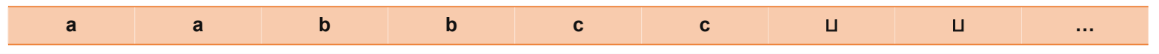
\includegraphics[width=0.9\linewidth]{../../images/nas.png}
    %\caption{caption}
    %\label{label}
\end{figure}
\noindent Abbiamo visto la definizione formale, ora vediamo a parole effettivamente come funziona la macchina.
La macchina ha diversi stati interni e inizia la computazione dallo stato iniziale, gli stati accettanti
terminano la computazione e accettano l'input, mentre gli stati rifiutanti terminano la computazione e 
e rifiutano l'input. La macchina può manipolare i simboli nel nastro della memoria interna e quelli dell'input.
La funzione di transizione associa ad ogni coppia di ($Q', \Gamma$) una terna ($q',\sigma',t$) dove:
\begin{itemize}
    \item $q'\in Q$ è il prossimo stato interno della macchina
    \item $\sigma' \in \Gamma$ è il simbolo che sovrascrive quello corrente
    \item $t \in \{ \leftarrow,\rightarrow, -  \}$ è lo spostamento della testina lungo il nastro che avviene dopo la scrittura,
    ovviamente $\leftarrow$ è uno spostamento a sinistra, $\rightarrow$ a destra e $-$ nessuno spostamento.
\end{itemize}








\noindent \textit{Esempio.} Vediamo prima un algoritmo che simula a parole il funzionamento di una macchina di Turing, poi vediamo la definizione formale della macchina.\\
Vogliamo che la macchina riconosca il linguaggio $\mathcal{L} = \{ a^n b^n c^n | n\ge 0 \}$\smallskip\\
Definiamo la macchina di Turing $M = \langle \Sigma, \Gamma, Q, \delta, q_0, q_{yes}, q_{no} \rangle$ come segue:
\begin{figure}[H]
    \centering  
    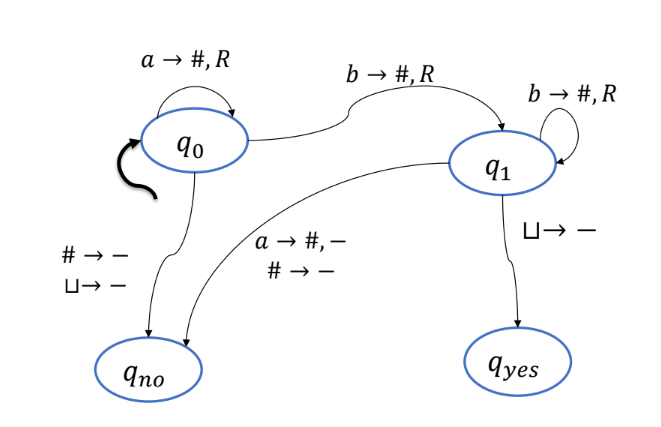
\includegraphics[width=0.6\linewidth]{../../images/tur.png}
    %\caption{caption}
    %\label{label}
\end{figure}
\begin{minipage}{0.45\textwidth}
    \begin{itemize}
        \item[-] $\Sigma = \{a, b\}$ Simboli di input
        \item[-] $\Gamma = \Sigma \cup \{\#, \sqcup\}$ Simboli del nastro
        \item[-] $Q = \{q_0, q_1, q_{yes}, q_{no}\}$ Insieme degli stati
    \end{itemize}
\end{minipage}
$\to$
\begin{minipage}{0.45\textwidth}
    \[
\begin{array}{|c|c|c|}
\hline
q & \sigma & \delta(q, \sigma) \\
\hline
q_0 & a & (q_0, \#, \rightarrow) \\
q_0 & b & (q_1, \#, \rightarrow) \\
q_0 & \# & (q_{no}, \#, -) \\
q_0 & \sqcup & (q_{no}, \sqcup, -) \\
q_1 & a & (q_{no}, \#, -) \\
q_1 & b & (q_1, \#, \rightarrow) \\
q_1 & \# & (q_{no}, \#, -) \\
q_1 & \sqcup & (q_{yes}, \sqcup, -) \\
\hline
\end{array}
\]
\end{minipage}\smallskip\\
Questi sono gli step che la macchina compie:
\begin{enumerate}[label=\arabic*.]
    \item \textbf{Leggi} il prossimo carattere $x$ dell'input
    \item Se $x = a$ Allora
    \begin{enumerate}[label=\arabic*.]
        \item \textbf{Sovrascrivi} tale occorrenza di $a$ con $\#_a$
        \item \textbf{Scorri} il nastro fino alla prossima occorrenza di $b$
        \begin{itemize}[label=--]
            \item Se incontri $y \in \{c, \#_c, \sqcup\}$ Allora \textcolor{red}{\textbf{rifiuta}}
            \item Altrimenti \textbf{sovrascrivi} tale occorrenza di $b$ con $\#_b$
        \end{itemize}
        \item \textbf{Scorri} il nastro fino alla prossima occorrenza di $c$
        \begin{itemize}[label=--]
            \item Se incontri $y \in \{a, \sqcup\}$ Allora \textcolor{red}{\textbf{rifiuta}}
            \item Altrimenti \textbf{sovrascrivi} tale occorrenza di $c$ con $\#_c$
        \end{itemize}
        \item \textbf{Torna} all'ultima occorrenza del simbolo $\#_a$
        \item \textbf{Torna} al passo 1 e avanza il nastro di 1
    \end{enumerate}
    \item Se $x \neq a$ Allora
    \begin{enumerate}[label=\arabic*.]
        \item \textbf{Scorri} fino a $\sqcup$, partendo dalla cella corrente
        \begin{itemize}[label=--]
            \item Se incontri $y \in \{a, b, c\}$ Allora \textcolor{red}{rifiuta}
            \item Altrimenti \textcolor{green}{\textbf{accetta}}
        \end{itemize}
    \end{enumerate}
\end{enumerate}


\subsection{Configurazioni}
\colorbox{SALZO}{\parbox{\dimexpr\linewidth-2\fboxsep}{\begin{definition}
   Sia $M = <\Sigma, \Gamma,Q,\delta,q_0,q_{yes},q_{no}>$ una macchina di Turing, una \textbf{configurazione} di $M$ è una 3-tupla
   $C= (\sigma,q,\tau)$ tale che:
   \begin{itemize}
    \item $\bm{\sigma}$ è una stringa sull'alfabeto $\Gamma$ (nastro a sinistra della testina)
    \item $\bm{\tau} \in \Gamma^*$ è una stringa sull'alfabeto $\Gamma$ (il primo simbolo di $\tau$ è il simbolo corrente)
    \item $\bm{q} \in Q$ è uno stato di $M$ (stato corrente della configurazione)
   \end{itemize}
\end{definition}}}\smallskip\\
Si utilizza la convenzione che a destra della testina il nastro a destra è \textbf{infinito}.\\
Una configurazione $C = (\sigma,q,\tau)$ di $M$ è detta:
\begin{itemize}
    \item \textbf{Accettante} (finale) se $q = q_{yes}$
    \item \textbf{Rifiutante} (finale) se $q = q_{no}$
    \item \textbf{Iniziale} se $q = q_0,\ \sigma = \epsilon$ (stringa vuota) e $\tau \in \Sigma^*$ ($\tau$ è una stringa dell'alfabeto in input)
\end{itemize}
Ora vediamo un esempio\smallskip\\
\textit{Esempio.} Prendiamo in esame la macchina di Turing nell'esempio della pagine precedente. Le seguenti sono delle possibili configurazioni:
\begin{itemize}
    \item[-] $(\epsilon, q_0, aa)$ è una configurazione \textbf{Iniziale} di $M$
    \item[-] $(abab, q_{yes}, abb \sqcup)$ è una configurazione \textbf{Accettante} di $M$
    \item[-] $(ab, q_{no}, ab \sqcup b)$ è una configurazione \textbf{Rifiutante} di $M$
    \item[-] $(\epsilon, q_1, aa)$ è una configurazione di $M$ (non iniziale, non finale)
    \item[-] $(\epsilon, q_0, aa\#)$ è una configurazione di $M$ (non è iniziale perché $\# \notin \Sigma$)
\end{itemize}




\subsection{Esecuzioni}
Sia $M = <\Sigma, \Gamma,Q,\delta,q_0,q_{yes},q_{no}>$ una macchina di Turing, siano $x,y,z \in \Gamma$ i simboli di nastro,
siano $\sigma,\tau \in \Gamma^*$ stringhe di simboli di nastro e siano $q,q'\in Q$, definiamo come avviene una \textbf{esecuzione}: \smallskip\\
\colorbox{SALZO}{\parbox{\dimexpr\linewidth-2\fboxsep}{\begin{definition}
   Una configurazione $C$ genera una configurazione $D$ in $M (C \Rightarrow_M D)$ se:
   \begin{itemize}
    \item $C = (\sigma y, q, x\tau)$, $D = (\sigma, q', yz\tau)$ e $\delta(q,x) = (q',z,\leftarrow)$ (movimento a sinistra)
    \item $C = (\epsilon, q, x\tau)$, $D = (\epsilon, q', z\tau)$ e $\delta(q,x) = (q',z,\leftarrow)$ (movimento a sinistra bloccato)
    \item $C = (\sigma, q, x\tau)$, $D = (\sigma z, q', \tau)$ e $\delta(q,x) = (q',z,\rightarrow)$ (movimento a destra)
    \item $C = (\sigma, q, x\tau)$, $D = (\sigma, q', z\tau)$ e $\delta(q,x) = (q',z,-)$ (nessun movimento)
   \end{itemize}
\end{definition}}}\smallskip\\
Ecco alcuni esempi:
\begin{itemize}
    \item Sia $C = (aab, q, bcc)$ e $\delta(q, b) = (q', \#, \leftarrow)$ allora $C$ genera $D = (aa, q', b\#cc)$
    \begin{itemize}
        \item[-] $C = (\sigma y, q, x\tau)$, $D = (\sigma, q', yz\tau)$ e $\delta(q, x) = (q', z, \leftarrow)$ (movimento a sinistra)
    \end{itemize}
    
    \vspace{0.3cm} % Aggiunge un po' di spazio per migliorare la leggibilità, simile alla foto
    
    \item Sia $C = (\epsilon, q, bcc)$ e $\delta(q, b) = (q', \#, \leftarrow)$ allora $C$ genera $D = (\epsilon, q', \#cc)$
    \begin{itemize}
        \item[-] $C = (\epsilon, q, x\tau)$, $D = (\epsilon, q', z\tau)$ e $\delta(q, x) = (q', z, \leftarrow)$ (movimento a sinistra bloccato)
    \end{itemize}
    
    \vspace{0.3cm}
    
    \item Sia $C = (aab, q, bcc)$ e $\delta(q, b) = (q', \#, \rightarrow)$ allora $C$ genera $D = (aab\#, q', cc)$
    \begin{itemize}
        \item[-] $C = (\sigma, q, x\tau)$, $D = (\sigma z, q', \tau)$ e $\delta(q, x) = (q', z, \rightarrow)$ (movimento a destra)
    \end{itemize}
    
    \vspace{0.3cm}
    
    \item Sia $C = (aab, q, \epsilon)$ e $\delta(q, \sqcup) = (q', \#, \rightarrow)$ allora $C$ genera $D = (aab\#, q', \epsilon)$
    \begin{itemize}
        \item[-] $C = (\sigma, q, x\tau)$, $D = (\sigma z, q', \tau)$ e $\delta(q, x) = (q', z, \rightarrow)$ (movimento a destra)
    \end{itemize}
    
    \vspace{0.3cm}
    
    \item Sia $C = (aab, q, bcc)$ e $\delta(q, b) = (q', \#, -)$ allora $C$ genera $D = (aab, q', \#cc)$
    \begin{itemize}
        \item[-] $C = (\sigma, q, x\tau)$, $D = (\sigma, q', z\tau)$ e $\delta(q, x) = (q', z, -)$ (nessun movimento)
    \end{itemize}
\end{itemize}
\noindent \textit{Osservazione.} Le macchine di Turing sono modelli computazionali \textbf{deterministici}, infatti per ogni possibile simbolo in input c'è un passaggio ben definito e non 
un insieme dei passaggi possibli.



\subsection{Linguaggi riconosciuti}
Come abbiamo fatto con gli automi, definiamo il linguaggio riconosciuto dalle macchine:\smallskip\\
\colorbox{SALZO}{\parbox{\dimexpr\linewidth-2\fboxsep}{\begin{definition}
   La macchina $M$ accetta/rifiuta l'input $\sigma \in \Sigma^*$ se esiste una sequenza finita di configurazioni $C_1,C_2,,...,C_n$ di $M$
   tale che le seguenti proprietà sono soddisfatte:
   \begin{itemize}
    \item $C_1 = (\epsilon,q_0,\sigma)$
    \item $C_n$ è una configurazione accettante o rifiutante 
    \item $C_i \Rightarrow_M C_{i+1}$ per ogni $i = 1,...,n-1$
   \end{itemize}
\end{definition}}}\smallskip\\
L'insieme $\bm{L(M)}$ delle stringhe che $M$ accetta è detto \textbf{linguaggio riconosciuto da M}.\smallskip\\
\textit{Esempio.} Sia $M = \langle \Sigma, \Gamma, Q, \delta, q_0, q_{yes}, q_{no} \rangle$ con $\Sigma = \{a, b, \#\}$, $\Gamma = \Sigma \cup \{\sqcup\}$, $Q = \{q_0, q_{yes}, q_{no}\}$
\[
\begin{array}{|c|c|c|}
\hline
q & \sigma & \delta(q, \sigma) \\
\hline
q_0 & a & (q_0, a, \rightarrow) \\
q_0 & b & (q_{yes}, b, -) \\
q_0 & \# & (q_{no}, \#, \leftarrow) \\
q_0 & \sqcup & (q_0, \sqcup, \rightarrow) \\
\hline
\end{array}
\]
La macchina $M$ \textbf{accetta} l'input $\bm{aab }\in \Sigma^*$ a causa di $(C_1, C_2, C_3, C_4)$
\begin{itemize}
    \item[-] La \textbf{configurazione iniziale} $C_1 = (\epsilon, q_0, aab)$ genera la configurazione $C_2 = (a, q_0, ab)$
    \item[-] La configurazione $C_2 = (a, q_0, ab)$ genera la configurazione $C_3 = (aa, q_0, b)$
    \item[-] La configurazione $C_3 = (aa, q_0, b)$ genera la \textbf{configurazione accettante} $C_4 = (aa, q_{yes}, b)$
\end{itemize}


\subsection{Macchine di Turing terminanti }
\colorbox{SALZO}{\parbox{\dimexpr\linewidth-2\fboxsep}{\begin{definition}
   Una macchina di Turing $M = <\Sigma, \Gamma,Q,\delta,q_0,q_{yes},q_{no}>$ è \textbf{terminante} se per ogni stringa $\sigma \in \Sigma^*$ abbiamo che $M$ accetta o rifiuta $\sigma$.
\end{definition}}}\medskip\\
\noindent Un linguaggio di stringhe $\mathcal{L}$ è detto \textbf{Turing Riconoscibile} se esiste una macchina di Turing $M$ che riconosce $\mathcal{L}$,
ovvero:
\[  \mathcal{L} = L(M)    \]
Inoltre un linguaggio $\mathcal{L}$ è detto \textbf{Turing Decidibile} se esiste un \textbf{decisore}, ovvero una macchina di Turing terminante $M$
che riconosce $\mathcal{L}$, ovvero come prima vale che $\mathcal{L} = L(M)$.\\
Queste definizioni sono necessarie poichè può accadere che se una macchina non finisce nè in uno stato accettante o nè rifiutante, può rimanere bloccata
in un ciclo infinito. \\Perciò definiamo anche cosa è una \textbf{macchina di Turing terminante}:\smallskip\\
\newpage
\subsection{Esercizio esempio}
Costruire una macchina di Turing che riconosca il seguente linguaggio:
\[    \mathcal{L} = \{  a^nb^nc^n |n \ge 0 \}        \]
\begin{figure}[H]
    \centering  
    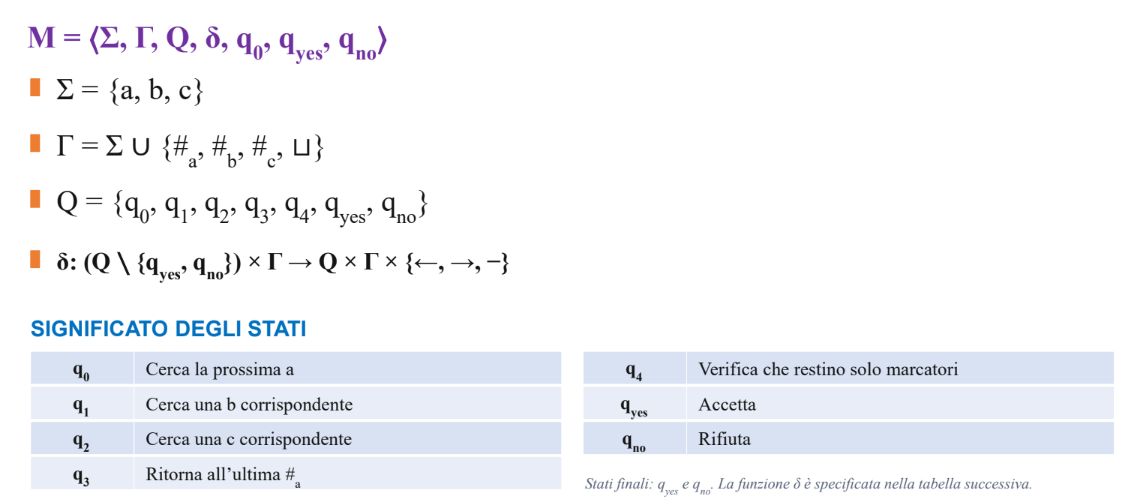
\includegraphics[width=0.9\linewidth]{../../images/est1.png}
    %\caption{caption}
    %\label{label}
\end{figure}
\begin{figure}[H]
    \centering  
    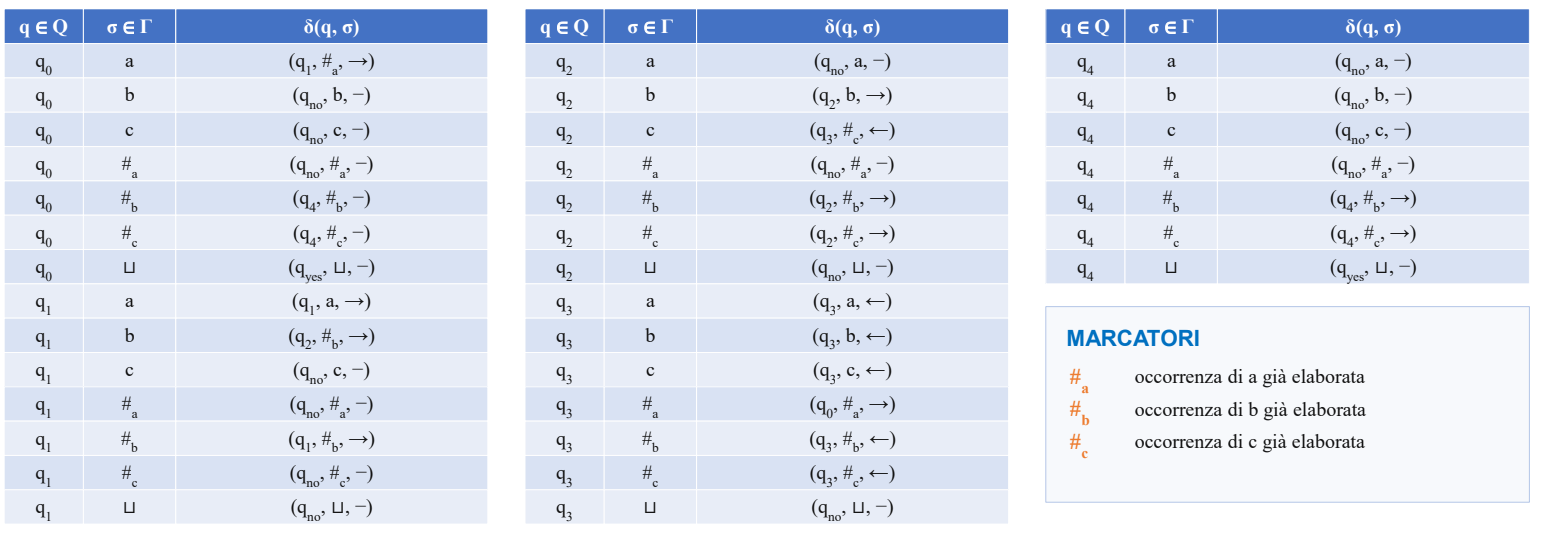
\includegraphics[width=0.9\linewidth]{../../images/est2.png}
    %\caption{caption}
    %\label{label}
\end{figure}



    